\chapter{Tổng quan về công nghệ và cơ sở lý thuyết}

Trong chương này, đồ án sẽ trình bày các công nghệ và khái niệm cơ bản liên quan đến việc xây dựng hệ thống co giãn tài nguyên và đồng thời mô tả những vấn đề còn tồn đọng cần phải giải quyết. Mục tiêu là cung cấp một cái nhìn tổng quan về các thành phần chính được sử dụng dụng trong hệ thống để làm cơ sở cho việc triển khai và đánh giá hệ thống trong lần lượt các chương tiếp theo 3, 4.

Nội dung chính của chương 2 bao gồm:
\begin{itemize}
    \item Apache Storm
    \item Docker
\end{itemize}

\section{Apache Storm}

Theo trang chủ Apache Storm \autocite{apachestorm}, đây là một nền tảng tính toán thời gian thực phân tán, mã nguồn mở, được thiết kế để xử lý các luồng dữ liệu liên tục. Nó cung cấp chức năng tương tự như Apache Hadoop nhưng được tối ưu hóa để luồng dữ liệu không giới hạn (unbounded streams of data), trong khi Hadoop xử lý dữ liệu theo lô (batch processing).

Apache Storm có sử dụng đơn giản, có thể được sử dụng bởi bất kỳ ngôn ngữ lập trình nào. Nhờ đó, Apache Storm có thể được áp dụng trong nhiều lĩnh vực, bao gồm: phân tích thời gian thực, học máy trực tuyến, tính toán liên tục, RPC phân tán, ETL và hơn thế nữa. Hệ thống này có khả năng xử lý dữ liệu với tốc độ cao, đạt hiệu suất trên một triệu bộ dữ liệu mỗi giây trên mỗi nút trong các thử nghiệm hiệu năng. Nó cũng cung cấp khả năng mở rộng, khả năng chịu lỗi và đảm bảo xử lý dữ liệu đồng thời cũng dễ cài đặt, triển khai và vận hành.

\subsection{Đôi nét về xử lý dữ liệu luồng}

Theo Rivery \autocite{rivery_batch_vs_stream}, xử lý luồng (Stream Processing) là phương pháp xử lý và phân tích dữ liệu liên tục, nơi dữ liệu được thu thập và phân tích ngay khi nó được tạo ra. Nhờ vậy, nó cho phép phản ứng ngay lập tức với các thay đổi, một yêu cầu thiết yếu cho các tác vụ đòi hỏi phải đưa ra quyết định nhanh.

So sánh với xử lý theo lô (Batch Processing):
\begin{itemize}
    \item \textbf{Xử lý dữ liệu:}
          \begin{itemize}
              \item Xử lý luồng: Xử lý dữ liệu liên tục, không ngừng nghỉ.
              \item Xử lý theo lô: Xử lý dữ liệu theo từng khối lớn, được xác định trước.
          \end{itemize}
    \item \textbf{Thời gian xử lý:}
          \begin{itemize}
              \item Xử lý luồng: Xử lý diễn ra trong thời gian thực, ngay khi dữ liệu được tạo ra.
              \item Xử lý theo lô: Xử lý diễn ra theo lịch trình cố định, không phải lúc dữ liệu được tạo ra.
          \end{itemize}
    \item \textbf{Độ phức tạp:}
          \begin{itemize}
              \item Xử lý luồng: Thường phức tạp hơn do yêu cầu xử lý liên tục và khả năng xảy ra các vấn đề về tính nhất quán.
              \item Xử lý theo lô: Thường đơn giản hơn, do dữ liệu được xử lý theo từng khối đã xác định.
          \end{itemize}
    \item \textbf{Độ trễ:}
          \begin{itemize}
              \item Xử lý luồng: Độ trễ thấp, cung cấp thông tin chi tiết ngay lập tức.
              \item Xử lý theo lô: Độ trễ cao hơn, thông tin chi tiết không có ngay lập tức.
          \end{itemize}
\end{itemize}

Các trường hợp sử dụng của xử lý luồng:
\begin{itemize}
    \item Phát hiện gian lận: Xác định các giao dịch hoặc hoạt động bất thường trong thời gian thực.
    \item Giám sát mạng: Theo dõi lưu lượng mạng và phát hiện các mối đe dọa bảo mật.
    \item Phát hiện xâm nhập: Phát hiện các hoạt động xâm nhập trái phép vào hệ thống.
\end{itemize}
Đặc biệt, xử lý luồng tỏ ra đặc biệt phù hợp để xử lý dữ liệu từ các thiết bị IoT, như nhiệt kế thông minh, công cụ theo dõi sức khỏe, cho phép phản xạ lập tức với các thay đổi trong môi trường xung quanh thiết bị.

\subsection{Các thành tố của cụm Apache Storm}

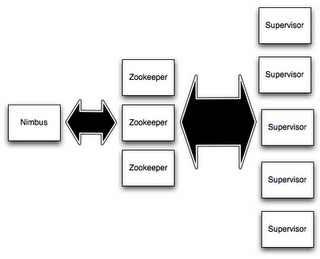
\includegraphics{storm-cluster.png}

Theo trang chủ Apache Storm \autocite{apachestorm}, các thành tố chính của cụm Apache Storm bao gồm: Nimbus, Supervisor, Zookeeper.

Có 2 loại nút trong cụm Storm: nút chủ (master node) và nút thực thi (worker node).

Nút chủ chạy tiến trình "nimbus", chúng chịu trách nhiệm phân phối mã (topology), gán các tác vụ cho các nút worker (Supervisor) và giám sát các lỗi quá trình thực thi của chúng.

Nút thực thi chạy tiên trình "supervisor", chịu trách nhiệm thực thi các phần của topology được gán, chạy hoặc dừng các tiến trình thực thi (worker process) khi cần thiết theo chỉ đạo bởi nút chủ.

Nút Zookeeper, chạy tiến trình "zookeeper", tuy các tiến trình này không được thiết kế dành riêng cho Apache Storm nhưng có vai trò đặc biệt, đóng vai trò điều phối viên giữa Nimbus và Supervisor. Thực tế rằng, cả Nimbus lẫn Supervisor đều là stateless và fail-fast nên có thể ví Zookeeper như trí nhớ của toàn bộ hệ thống. Zookeeper có trách nhiệm lưu trữ thông tin về trạng thái của các nút Nimbus và Supervisor trong cụm Storm. Thông tin này bao gồm trạng thái hoạt động, thông tin cấu hình, và các chi tiết liên quan đến các Topology đang chạy. Thông qua Zookeeper, Nimbus và các Supervisor có thể giao tiếp với nhau một cách dễ dàng, nhất quán, hiệu quả.

Nhờ sử dụng kiến trúc master-slave điển hình đồng thời lưu trữ dữ liệu tại các nút Zookeeper, hệ thống cụm Storm có những ưu điểm tuyệt vời:
\begin{itemize}
    \item có sự ổn định đáng kinh ngạc.
    \item Trong một cụm, chỉ yêu cầu một nút chủ duy nhất do nút này là stateless (không lưu trữ dữ liệu).
    \item Tương tự như nút chủ, các nút thực thi cũng là stateless giúp tất cả chúng có thể được dễ dàng tái khởi động khi gặp lỗi, sự cố trong quá trình chạy
\end{itemize}

\section{Docker}

Theo \autocite{docker}, Docker là một nền tảng mã nguồn mở cho phát triển, phân phối và chạy các ứng dụng. Dockers cho phép người dùng tách biệt các ứng dụng của họ khỏi cơ sở hạ tầng giúp công việc phân phối phần mềm nhanh chóng. Với Docker, người dùng có thể quản lý cơ sở hạ tầng theo cùng cách họ quản lý các ứng dụng. Bằng cách tận dụng lợi thế khi áp dụng Docker vào công việc phân phối, kiểm thử và triển khai mã nguồn, người dùng có thể giảm đáng kể thời gian giữa công đoạn viết code với công đoạn triển khai trong thực tế.

\subsection{Nền tảng Docker}

Docker cung cấp khả năng đóng gói và chạy ứng dụng trong môi trường cô lập lỏng lẻo (loosely isolated environment) được gọi là container. Sự cô lập và bảo mật này cho phép người dùng chạy nhiều container đồng thời trên cùng một máy chủ. Các container rất gọn nhẹ nhưng bao gồm đầy đủ các thành phần cần thiết để chạy một ứng dụng, do đó người dùng không cần phải dựa trên các thành phần đã được cài đặt trên máy chủ. Người dùng có thể chia sẻ các container và chắc chẳn rằng tất cả những người nhận đều sẽ thu được cùng một container có cách hoạt động y hệt.

Docker cung cấp bộ công cụ và nền tảng để kiểm soát vòng đời của các container.

\begin{itemize}
    \item Phát triển ứng dụng của người dùng và các thành phần phụ trợ sử dụng container.
    \item Các container trở thành đơn vị để phân phối và kiểm thử ứng dụng của người dùng.
    \item Khi người dùng sẵn sàng, triển khai ứng dụng của người dùng trong môi trường kinh doanh, dưới hình thức một container hoặc dịch vụ điều phối (orchestrated service). Tất cả đều có cùng cách hoạt động bất kể là môi trường kinh doanh của người dùng là trung tâm dữ liệu cục bộ, nền tảng điện toán đám mây hay là sự kết hợp của hai môi trường trên.
\end{itemize}

\subsection{Dùng Docker để làm gì?}

\subsubsection{Phân phối ứng dụng một cách nhanh chóng, đồng nhất}

Docker đẩy nhanh vòng đời phát triển bằng cách cho phép các lập trình viên hoạt động trong một môi trường đã được chuẩn hóa sử dụng các container cục bộ - thứ cũng sẽ đồng thời cung cấp các ứng dụng và dịch vụ của bạn. Các container cực kỳ phù hợp với các quy trình CI/CD.

Tất cả các công đoạn trong vòng đời phát triển sản phẩm đều sẽ được tăng tốc thông qua Docker:
\begin{itemize}
    % TODO: Tại sao lại nhanh hơn
    \item Lập trình viên viết mã nguồn và chia sẻ thành quả với các đồng nghiệp sử dụng container của Docker.
    \item Lập trình viên dùng Docker để xây dựng môi trường kiểm thử để chạy các bộ kiểm thử cả tự động lẫn thủ công.
    \item Khi lập trình viên tìm thấy lỗi, họ có thể sửa chúng trong môi trường phát triển rồi tái triển khai chúng lên môi trường kiểm thử để kiểm thử và đánh giá.
    \item Khi hoàn thành kiểm thử, phân phối bản sửa lỗi đến với khách hàng cũng đơn giản như việc triển khai trên môi trường kinh doanh.
\end{itemize}

\subsubsection{Triển khai đáp ứng và co dãn tài nguyên}

Hiện nay, một sáng kiến có tên The Open Container Initiative (OCI) \autocite{opencontainerinitiative}, được vận hành dưới sự bảo trợ của Linux Foundation \autocite{linuxfoundation} % TODO:
đóng vai trò quan trọng trong hệ sinh thái container hiện đại. Mục đích chính của OCI là phát triển các tiêu chuẩn ngành cho định dạng container và phần mềm thực thi container cho tất cả các nền tảng có sử dụng công nghệ container. Cụ thể là, sáng kiến này sẽ đảm bảo rằng công nghệ container có thể hoạt động đa nền tảng. Điều này có nghĩa là container được xây dựng bởi một bộ công cụ sẽ có thể chạy trên một bộ công cụ khác, giảm thiểu sự phụ thuộc vào nhà cung cấp.

Kết hợp với khả năng tạo môi trường độc lập thống nhất giữa các nền tảng thì các hệ thống được xây dựng dựa trên nền tảng container của Docker hay rộng ra là công nghệ container sẽ cho phép tính di động cao. Hiện nay, các container có thể chạy trên máy tính laptop của lập trình viên, trên máy ảo hoặc máy vật lý trong trung tâm dữ liệu, trên nền tảng điện toán đám mây hoặc là hệ thống kết hợp nhiều mô hình.

Bản chất linh hoạt và gọn nhẹ của Docker còn giúp chúng dễ dàng điều phối khối lượng công việc, tăng/giảm các ứng dụng, dịch vụ nhanh chóng gần như theo thời gian thực.

\subsubsection{Triển khai nhiều khối lượng công việc hơn trên cùng một phần cứng không đổi}

Docker nhẹ và nhanh, có thể coi là một giải pháp thay thế khả thi và tối ưu tài nguyên so với các máy ảo dựa trên công nghệ ảo hóa, nhờ đó người dùng có thể sử dụng tài nguyên hệ thống hiệu quả hơn nhưng vẫn đảm bảo được hiệu suất, khả năng vận hành.

\subsection{Kiến trúc}
Docker sử dụng mô hình kiến trúc client-server. Docker client gửi yêu cầu đến Docker daemon, thành phần xử lý toàn bộ các phần việc xây dựng, chạy và phân phối container. Client và daemon có thể chạy trên cùng một máy hoặc kết nối từ xa qua mạng. Chúng giao tiếp qua REST API thông qua socket UNIX hoặc giao diện mạng. Một thành phần quan trọng khác của Docker client là Docker Compose giúp quản lý ứng dụng gồm nhiều container (sẽ được đề cập đến sau đây).

\begin{center}
    \begin{figure}
        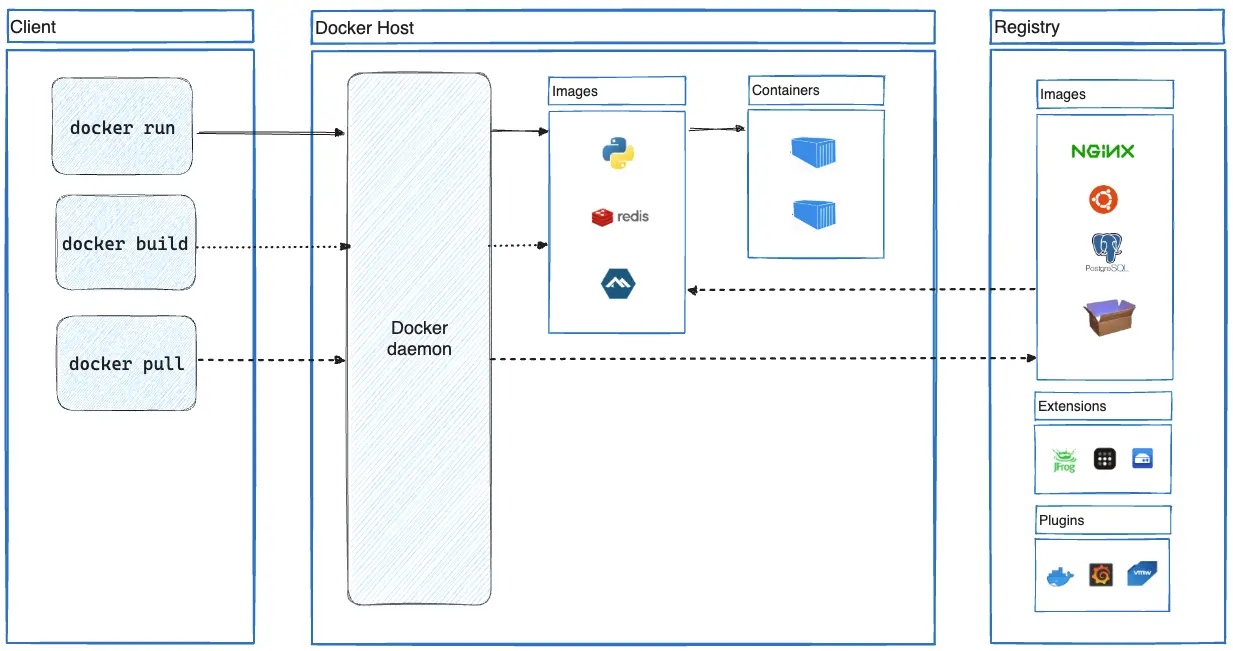
\includegraphics[width=\textwidth]{docker-architecture.png}
        \caption{Kiến trúc Docker}
    \end{figure}
\end{center}


\subsubsection{Tiến trình nền của Docker}

Tiến trình nền của Docker - dockerd lắng nghe các yêu cầu Docker API và quản lý các đối tượng của Docker như image, container, mạng và không gian lưu trữ. Tiến trình nền này có thể tương tác với các tiến trình khác để quản lý các dịch vụ của Docker.

\subsubsection{Docker client}

Công cụ dòng lệnh `\texttt{docker}` là phương pháp chính mà người dùng sử dụng để tương tác với Docker. Khi người dùng gửi các lệnh như `\texttt{docker run}`, client sẽ gửi lệnh này đến `\texttt{dockerd}`, tiến trình nền như đã đề cập, sẽ thực hiện các công việc cần thiết để chạy container. Công cụ dòng lệnh `\texttt{docker}` sẽ sử dụng Docker API.

\subsection{Các đối tượng của Docker}

\subsubsection{Images}

Đây là bản hướng dẫn chỉ đọc (read-only template) chưa các hướng dẫn để tạo container. Thông thường một image sẽ dựa trên image khác với một số thay đổi. Có thể sử dụng các image đã được tạo sẵn bởi những người, tổ chức khác đã công bố trên docker registry hoặc người dùng có thể tự xây dựng một bản của riêng.

Để tạo image của riêng mình, mỗi người dùng có thể tạo tệp Dockerfile với cú pháp đơn giản để định nghĩa các bước cần thiết để tạo image và chạy chúng. Mỗi chỉ dẫn trong Dockerfile tạo thành một lớp trong image. Khi người dùng thay đổi Dockerfile và tái xây dựng image, chỉ các lớp đã bị thay đổi mới bị tái xây dựng. Đây là nguyên nhân khiến cho các image rất nhẹ, nhỏ gọn và nhanh khi so sánh với các công nghệ ảo hóa.

\subsubsection{Containers}

Container là bản thể chạy được của image. Người dùng có thể tạo, khởi động, dừng, chuyển, xóa một container thông qua Docker API hoặc CLI. Người dùng có thể kết nối một container với một hoặc nhiều hơn các mạng, gắn các công cụ lưu trữ cho nó hoặc tạo một image mới dựa trên trạng thái hiện tại của container.

Theo mặc định, một container được phân tách khá độc lập so với các container khác và cả máy chủ đang chạy chúng, tuy nhiên tất cả các yếu tố như mạng của của container, thiết bị lưu trữ hoặc các hệ thống con bên trong đều có thể được tùy chỉnh bởi người dùng.

Do vậy, các container mở ra khả năng triển khai nhất quán, dễ dàng và hiệu quả trên mọi hạ tầng mà nó được triển khai.